
\section{Results}

\subsubsection{Figures of merit}

\begin{table*}[]
\caption{Technology FOM's}
\label{tab:techFOM}
\resizebox{\textwidth}{!}{%
\begin{tabular}{|l|l|l|}
\hline
cost hardware, software & USD & cost or hardware rent to provide coverage of needed area with normal operating accuracy \\ \hline
accuracy & m & accuracy of localization, difference between real position and measurements \\ \hline
cost & f(USD/sqm) & the cost itself cannot be directly compared because of different types of implementation. Instead, the overall cost presented in several roadmaps is shown. \\ \hline
range & m & Not important factor, complexity and scalability are affected by this factor. Not representative, because of different types of implementation. Excluded from FOM's \\ \hline
additional requirements & \begin{tabular}[c]{@{}l@{}}USD;\\ year\end{tabular} & If yes, product is not applicable until they are not solved. Not implemented into model, technologies with additional requirements are mot mapped. (Infrastructure Requirements, Impacts and Notes) \\ \hline
Scalability & low/med/high & range of scalability, important factor to consider in strategy choice \\ \hline
Complexity & low/med/high & range of complexity, important factor to consider in strategy choice \\ \hline
Robustness &  & additional information of what affect the performance of technology \\ \hline
\end{tabular}%
}
\end{table*}

Lower figures in table are affecting the technology choise, but cannot be added into model, so they are not considered as the figures of merit, but listed in table to explain the reason of excluding them.

\begin{table}[]
\caption{Product FOM's}
\label{tab:ProductFOM}
\begin{tabular}{lll}
accuracy & m & accuracy of localization, RMS error between real position and measurements \\
development time & month & time to develop the product based on technology with specified accuracy
\end{tabular}%
\end{table}

We focus on the figures of merit which are important for product development, and we use product FOM's mostly\ref{tab:ProductFOM}.

\begin{table*}[]
\caption{Performance of different technologies from the indoor positioning competition}
\label{tab:my-competition}
\resizebox{\textwidth}{!}{%
\begin{tabular}{|l|l|l|l|l|}
\hline
Team & Technical Approach & dev.time & RMS error & Team’s Affiliation \\ \hline
1 & 2.4GHz Phase Offset & 60 & 0.72 & Lambda:4 Entwicklungen \\ \hline
2 & WiFi+Modulated LEDs & 12 & 2.04 & MSR Asia \\ \hline
3 & 2.4GHz Time-of-Flight & 72 & 2.03 & Freie Univ. Berlin \\ \hline
4 & Ultrasonic Time-of-Flight &  & 2.09 & CMU \\ \hline
5 & IR/Radio Time-of-Flight & 18 & 2.35 & Rutgers \\ \hline
6 & 2.4GHz Time-of-Flight & 5 & 2.58 & Wroclaw Univ. of Tech. MT-Silesia Sp. \\ \hline
7 & WiFi+Bluetooth+IMU & 24 & 2.72 & NextoMe \\ \hline
8 & Modulated Magnetic Signals & 24 & 3.83 & Univ. of Oxford \\ \hline
9 & SDR Time-of-Flight & 4 & 3.87 & Humboldt Univ. of Berlin \\ \hline
10 & Modulated Magnetic Signals & 90 & 3.96 & DFKI \\ \hline
11 & 2.4GHz Phase Offset & 24 & 4.04 & Greina Technologies \\ \hline
12 & WiFi+Sound Time-of-Flight & 12 & 8.91 & Xian Jiaotong Univ. \\ \hline
13 & Steerable Antennas ToF & 12 & 10.22 & I.E.C.S. \\ \hline
14 & Bayesian Filter + WiFi Fingerprinting & 96 & 1.56 & Cork Institute of Technology \\ \hline
15 & WiFi+IMU Fingerprinting + Neural Network & 36 & 1.96 & Univ. of Cyprus/Cywee \\ \hline
16 & WiFi Fingerprinting + Neural Network & 12 & 2.22 & Nanyang Tech. Univ. \\ \hline
17 & WiFi+IMU Fingerprinting & 9 & 2.81 & Ubee S.A. \\ \hline
18 & WiFi+IMU Fingerprinting + Particle Filter & 24 & 3.19 & MSR Asia \\ \hline
19 & WiFi Time-of-Flight + Adaptive Filter & 12 & 3.47 & ETH/IMDEA/Armasuisse \\ \hline
20 & WiFi+IMU+Maps + Conditional Random Fields & 12 & 3.71 & Univ. of Oxford \\ \hline
21 & WiFi+Magnetic Fingerprinting + Particle Filter & 12 & 4.86 & Nanyang Tech. Univ. \\ \hline
22 & WiFi+IMU Fingerprinting + Clustering/Decision Trees & 3 & 5.23 & Tata Consulting Services \\ \hline
\end{tabular}%
}
\end{table*}

Technological limits

3 types: radio (distance), image (angle), fingerprinting (position).

Radio (multilateration, distance measurement), fingerprinting: noise level, wave reflections, sensor errors are main limitations.
Because of noise, the technology limit can’t be reached, only on frequencies where is no external noise, wave reflections - scanning error depends on geometry of signal way.
Image based: accuracy/precision of localisation depends on camera angle resolution. Because trilateration with camera is not possible, error is a linear function of range.



\subsection{State of the art}

\begin{table*}[h!]
\caption{technology comparison}
\label{tab:tech-comparison}
\resizebox{\textwidth}{!}{%
\begin{tabular}{|l|l|l|l|l|l|}
\hline
\textbf{IPS Technology}       & \textbf{Type}  & \textbf{Accuracy, m} & \textbf{Scalability} & \textbf{Complexity} & \textbf{Cost} \\ \hline
Geomagnetic                   & fingerprinting & 2                    & Low                  & Low                 & Very Low      \\ \hline
Photo                         & camera         & 1-10                 & Low                  & High                & High          \\ \hline
Barcodes                      & camera         & 1-10                 & Medium               & Low                 & Low           \\ \hline
Video, AR                     & camera         & 1-10                 & Low                  & High                & High          \\ \hline
Bluetooth Low Energy (BLE)    & Radio          & 1-3                  & High                 & Medium              & Medium        \\ \hline
RFID, Active                  & Radio          & 1-10                 & Medium               & Medium              & Medium        \\ \hline
RFID, Passive                 & Radio          & 1-10                 & Medium               & Medium              & Medium        \\ \hline
Wi-Fi                         & Radio          & 5-10                 & High                 & Medium              & Low           \\ \hline
Ultra Wide Band (UWB)         & Radio          & 0.15-0.5             & Low                  & Medium              & Medium to Low \\ \hline
Zigbee                        & Radio          & 3-5                  & Low                  & Low                 & Low           \\ \hline
FM                            &                & 2-4                  & Low                  & Low                 & Low           \\ \hline
Lighting-Based – Infrared LED & Lighting       & 0.15-3               & Low                  & Low                 & Low           \\ \hline
Lighting-Based – Visible LED  & Lighting       & 0.3-3                & Low                  & Low                 & Low           \\ \hline
Audible                       & sonic          & 0.5                  & Low                  & Low                 & Low           \\ \hline
Ultrasound                    & sonic          & 0.05-0.25            & Low                  & Medium              & Low to Medium \\ \hline
Inertial                      & supplementary  &                      & Low                  & Low                 &               \\ \hline
Pressure                      & supplementary  &                      &                      &                     &               \\ \hline
GPS                           & supplementary  & 6-10                 & Low                  & High                &               \\ \hline
\end{tabular}%
}
\end{table*}


\subsubsection{Positioning}
% companies positioning on market

We have to find products of this companies and other popular products to provide the landscape of market.


Number of patents is a valuable metric but it doesn't show us a value of patent, for example, Indooratlas OY obtain patents for magnetic fingerprinting technology which are more valuable now. Some huge companies such as Google LLC and Hitachi are not properly listed. They obtain higher number of patents that shown here, but all of them are not related to indoor navigation, so they are excluded from analysis. Excluding several companies is possible because best products are well known and we want to map products especially.

\cite{Security} It provides information about relative accuracy, mobile device battery usage and other system performance factors to help support early IPS planning and preliminary product evaluation.

\cite{Mautz2012IndoorPT}

IndoorAtlas research of 2016\cite{IPTrise} is a market landscape, which covers most popular technologies, market drivers and future trends. The paper covers adoption and drivers of indoor positioning systems, perspectives of geomagnetic indoor positioning.

Paper \cite{Brena2017} present a comparison of indoor positioning approaches.

% \cite{Kj_fingerprinting, Ashraf_deepnn, Li_geomagnetic, Mautz2012IndoorPT, 8859264, Infsoft_wp}

\begin{table}[]
\caption{Product index}
\label{tab:productstolink}
\begin{tabular}{|l|l|}
\hline
 & Products \\ \hline
P1 & Mapsted navigation deluxe \\ \hline
P2 & HERE Indoor Positioning (SDK \& radio mapper) \\ \hline
P3 & IndoorAtlas \\ \hline
P4 & VisioGlobe indoor navigation \\ \hline
P5 & Google VPS (visual positioning system) \\ \hline
\end{tabular}%
\end{table}

% Please add the following required packages to your document preamble:
% \usepackage{graphicx}
\begin{table}[]
\caption{Techologies index}
\label{tab:techindex}
\begin{tabular}{|l|l|}
\hline
index & sensors \\ \hline
T1 & GSM / 3G / 4G (LTE) \\ \hline
T2 & compass, magnetic fields \\ \hline
T3 & Wi-Fi \\ \hline
T4 & Bluetooth \\ \hline
T5 & accelerometer, gyroscope, pedometer \\ \hline
T6 & UWB antennas \\ \hline
T7 & Barometer \\ \hline
T8 & Camera \\ \hline
T9 & RFID, NFC, QR code \\ \hline
\end{tabular}%
\end{table}

We use the linking grid to map products \ref{tab:productstolink} to technologies \ref{tab:techindex}. To make table more compact, we use indexes.  

\begin{table*}[ht]
\caption{Technology comparison. Linking grid.}
\label{tab:linking_grid}
\resizebox{\textwidth}{!}{%
\begin{tabular}{lllllllllll|l|l|l|l|l|}
\cline{12-16}
 &  &  &  &  &  &  &  &  &  &  & \multicolumn{5}{l|}{Products} \\ \cline{12-16} 
 &  &  &  &  &  &  &  &  &  &  & \multicolumn{4}{l|}{current} & future \\ \cline{11-16} 
 &  &  &  &  &  &  &  &  & \multicolumn{1}{l|}{} & Markets & p1 & p2 & p3 & p4 & p5 \\ \cline{11-16} 
 &  &  &  &  &  &  &  & \multicolumn{2}{l}{} & positioning & x & x & x & x & x \\ \cline{11-16} 
 &  &  &  &  &  &  &  &  & \multicolumn{1}{l|}{} & marketing & x &  & x &  & x \\ \cline{11-16} 
 &  &  &  &  &  &  &  &  & \multicolumn{1}{l|}{} & analytics &  &  & x & x & x \\ \cline{11-16} 
 &  &  &  &  &  &  &  &  &  &  &  &  &  &  &  \\ \cline{2-16} 
\multicolumn{1}{l|}{} & \multicolumn{9}{l|}{Technologies} &  &  &  &  &  &  \\ \cline{2-16} 
\multicolumn{1}{l|}{} & \multicolumn{1}{l|}{T1} & \multicolumn{1}{l|}{T2} & \multicolumn{1}{l|}{T3} & \multicolumn{1}{l|}{T4} & \multicolumn{1}{l|}{T5} & \multicolumn{1}{l|}{T6} & \multicolumn{1}{l|}{T7} & \multicolumn{1}{l|}{T8} & \multicolumn{1}{l|}{T9} & Processes &  &  &  &  &  \\ \cline{2-16} 
\multicolumn{1}{l|}{} & \multicolumn{1}{l|}{x} & \multicolumn{1}{l|}{x} & \multicolumn{1}{l|}{x} & \multicolumn{1}{l|}{} & \multicolumn{1}{l|}{} & \multicolumn{1}{l|}{} & \multicolumn{1}{l|}{} & \multicolumn{1}{l|}{x} & \multicolumn{1}{l|}{x} & geofencing &  &  & x &  & x \\ \cline{2-16} 
\multicolumn{1}{l|}{} & \multicolumn{1}{l|}{} & \multicolumn{1}{l|}{} & \multicolumn{1}{l|}{x} & \multicolumn{1}{l|}{x} & \multicolumn{1}{l|}{} & \multicolumn{1}{l|}{x} & \multicolumn{1}{l|}{} & \multicolumn{1}{l|}{} & \multicolumn{1}{l|}{x} & asset tracking &  &  & x & x &  \\ \cline{2-16} 
\multicolumn{1}{l|}{} & \multicolumn{1}{l|}{x} & \multicolumn{1}{l|}{x} & \multicolumn{1}{l|}{x} & \multicolumn{1}{l|}{x} & \multicolumn{1}{l|}{x} & \multicolumn{1}{l|}{} & \multicolumn{1}{l|}{x} & \multicolumn{1}{l|}{x} & \multicolumn{1}{l|}{} & human real-time positioning & x & x & x & x & x \\ \cline{2-16} 
\multicolumn{1}{l|}{} & \multicolumn{1}{l|}{} & \multicolumn{1}{l|}{x} & \multicolumn{1}{l|}{x} & \multicolumn{1}{l|}{x} & \multicolumn{1}{l|}{} & \multicolumn{1}{l|}{} & \multicolumn{1}{l|}{} & \multicolumn{1}{l|}{} & \multicolumn{1}{l|}{} & queue management &  &  & x & x &  \\ \cline{2-16} 
\multicolumn{1}{l|}{} & \multicolumn{1}{l|}{} & \multicolumn{1}{l|}{} & \multicolumn{1}{l|}{x} & \multicolumn{1}{l|}{} & \multicolumn{1}{l|}{x} & \multicolumn{1}{l|}{x} & \multicolumn{1}{l|}{x} & \multicolumn{1}{l|}{} & \multicolumn{1}{l|}{x} & Sensor Fusion SLAM &  &  & x &  &  \\ \cline{2-16} 
\multicolumn{1}{l|}{} & \multicolumn{1}{l|}{x} & \multicolumn{1}{l|}{x} & \multicolumn{1}{l|}{x} & \multicolumn{1}{l|}{x} & \multicolumn{1}{l|}{x} & \multicolumn{1}{l|}{x} & \multicolumn{1}{l|}{x} & \multicolumn{1}{l|}{x} & \multicolumn{1}{l|}{} & map creation & x & x & x & x & x \\ \cline{2-16} 
\multicolumn{1}{l|}{} & \multicolumn{1}{l|}{} & \multicolumn{1}{l|}{} & \multicolumn{1}{l|}{} & \multicolumn{1}{l|}{} & \multicolumn{1}{l|}{} & \multicolumn{1}{l|}{} & \multicolumn{1}{l|}{} & \multicolumn{1}{l|}{} & \multicolumn{1}{l|}{} & Product phase &  &  &  &  &  \\ \hline
\multicolumn{1}{|l|}{mature} & \multicolumn{1}{l|}{} & \multicolumn{1}{l|}{} & \multicolumn{1}{l|}{} & \multicolumn{1}{l|}{x} & \multicolumn{1}{l|}{} & \multicolumn{1}{l|}{} & \multicolumn{1}{l|}{} & \multicolumn{1}{l|}{} & \multicolumn{1}{l|}{} & Research &  &  & x & x & x \\ \hline
\multicolumn{1}{|l|}{growth} & \multicolumn{1}{l|}{} & \multicolumn{1}{l|}{} & \multicolumn{1}{l|}{x} & \multicolumn{1}{l|}{} & \multicolumn{1}{l|}{x} & \multicolumn{1}{l|}{x} & \multicolumn{1}{l|}{} & \multicolumn{1}{l|}{x} & \multicolumn{1}{l|}{} & Development & x & x & x & x & x \\ \hline
\multicolumn{1}{|l|}{emerging} & \multicolumn{1}{l|}{} & \multicolumn{1}{l|}{x} & \multicolumn{1}{l|}{} & \multicolumn{1}{l|}{} & \multicolumn{1}{l|}{} & \multicolumn{1}{l|}{} & \multicolumn{1}{l|}{} & \multicolumn{1}{l|}{} & \multicolumn{1}{l|}{} & Delivery &  &  & x & x &  \\ \hline
\multicolumn{1}{|l|}{declining} & \multicolumn{1}{l|}{x} & \multicolumn{1}{l|}{} & \multicolumn{1}{l|}{} & \multicolumn{1}{l|}{} & \multicolumn{1}{l|}{} & \multicolumn{1}{l|}{} & \multicolumn{1}{l|}{x} & \multicolumn{1}{l|}{} & \multicolumn{1}{l|}{x} & Support & x & x & x & x &  \\ \hline
\end{tabular}%
}
\end{table*}

In linking grid \ref{tab:linking_grid}, we map technologies to possible processes in indoor positioning systems. For each technology, we identify the technology adoption or readiness level in simplest form. After that, for each process, we mark all possible technologies involved. Then we mark products to markets and identify which processes are involved into each product, on which markets the product is positioned and what the level of this product on the market. 


\subsubsection{Patents}

\begin{figure}[h]
    \centering
    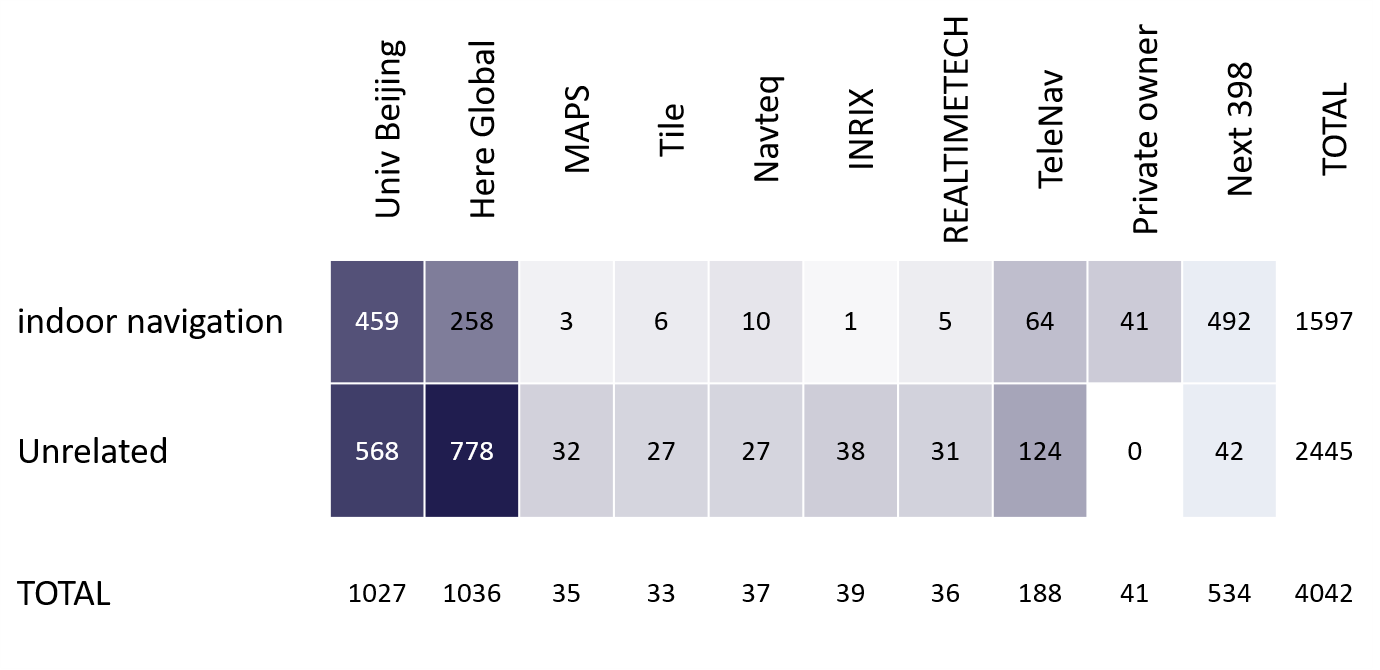
\includegraphics[width=0.48\textwidth]{img/patents/Patenting2.png}
    \caption{Portfolio size: Active patent families, by organisation and technology. Currently active patent families (granted or pending) by organisation and technology.}
    \label{fig:Patent-families2}
\end{figure}

In patent research of current field, we use patent classifier with the training set of 590 positive and 136 negative patents marked.
Using this classifier and AI patent platform cipher.ai, we do the organisation search which is presented on \ref{fig:Patent-families2}
. On the Figure \ref{fig:Patent-families2} category of "Unrelated" is the category of patents that does not fit the classifier.

\begin{figure}[h]
    \centering
    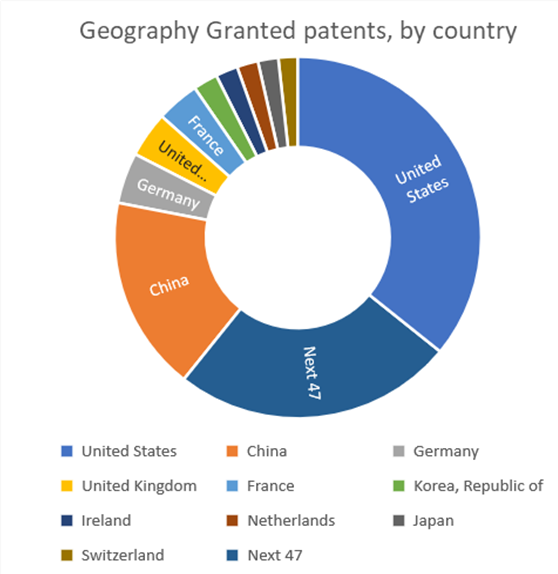
\includegraphics[width=0.48\textwidth]{img/patents/Granted patents by country and organisation.png}
    \caption{}
    \label{fig:Patent-u}
\end{figure}



\begin{figure*}[h]
    \centering
    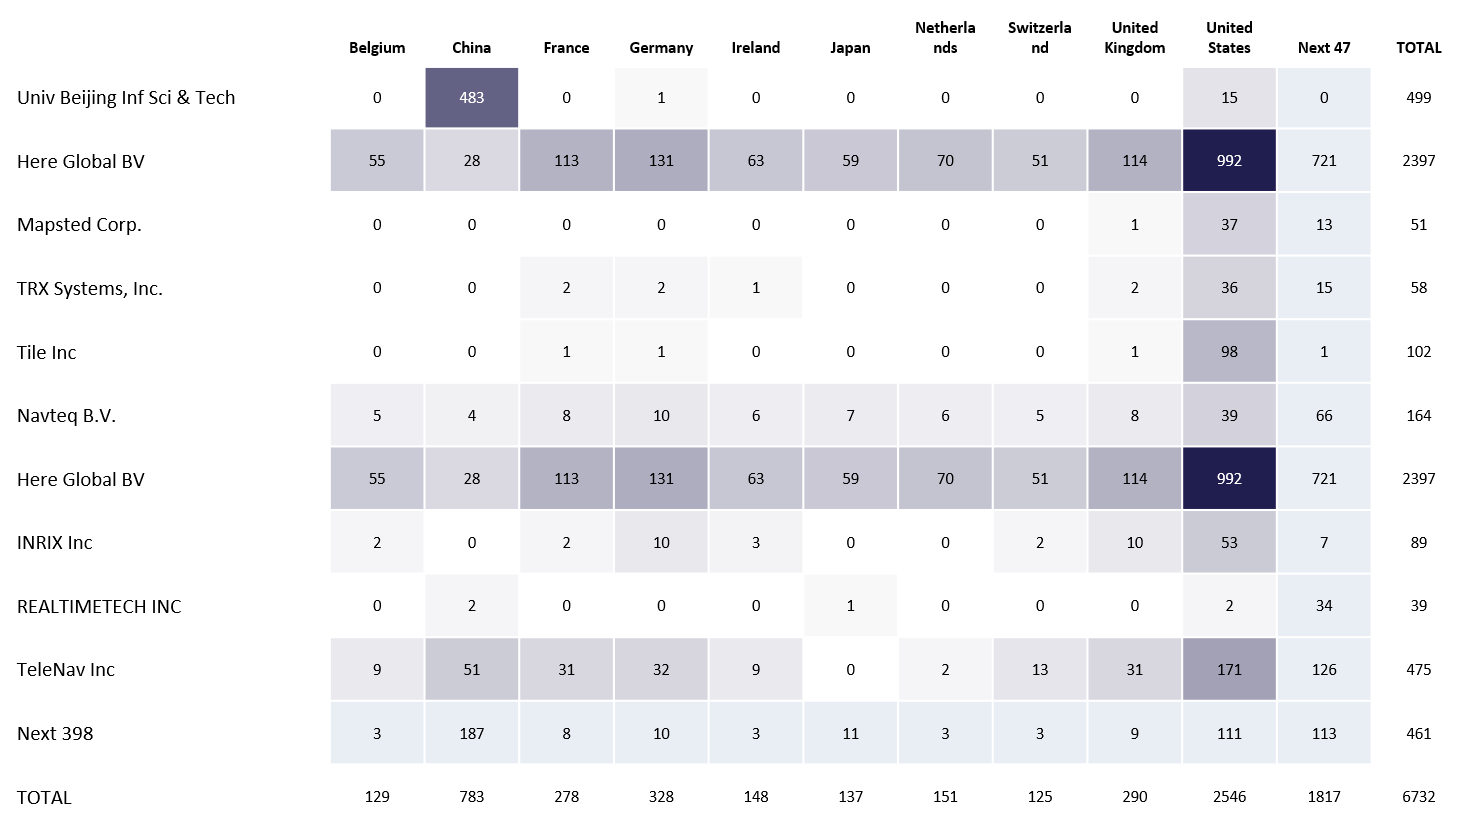
\includegraphics[width=\textwidth]{img/patents/Geography Granted patents by country and organisation.png}
    \caption{Geography: Granted patents, by country and organisation
Currently active and granted individual patents per country, by organisation.}
    \label{fig:Granted-patents-by-coutry}
\end{figure*}



\begin{table*}[]
\caption{Portfolio size: Active patent families, by organization and technology}
\label{tab:patents-scope}
\resizebox{\textwidth}{!}{%
\begin{tabular}{lllllllllll}
 & Univ Beijing & Here Global & MAPS & Tile & Navteq & REALTIMETECH & TeleNav & Private owner & Next 398 & TOTAL \\
indoor navigation & 459 & 258 & 3 & 6 & 10 & 5 & 64 & 41 & 492 & 1597 \\
Unrelated & 568 & 778 & 32 & 27 & 27 & 31 & 124 & 0 & 42 & 2445 \\
TOTAL & 1027 & 1036 & 35 & 33 & 37 & 36 & 188 & 41 & 534 & 4042
\end{tabular}%
}
\end{table*}


\begin{table*}[]
\caption{Geography: Granted patents, by country and organization}
\label{tab:patents-map}
\resizebox{\textwidth}{!}{%
\begin{tabular}{lllllllllllll}
 & Belgium & China & France & Germany & Ireland & Japan & Netherlands & Switzerland & United Kingdom & United States & Next 47 & TOTAL \\
Univ Beijing Inf Sci \& Tech & 0 & 483 & 0 & 1 & 0 & 0 & 0 & 0 & 0 & 15 & 0 & 499 \\
Here Global BV & 55 & 28 & 113 & 131 & 63 & 59 & 70 & 51 & 114 & 992 & 721 & 2397 \\
Mapsted Corp. & 0 & 0 & 0 & 0 & 0 & 0 & 0 & 0 & 1 & 37 & 13 & 51 \\
TRX Systems, Inc. & 0 & 0 & 2 & 2 & 1 & 0 & 0 & 0 & 2 & 36 & 15 & 58 \\
Tile Inc & 0 & 0 & 1 & 1 & 0 & 0 & 0 & 0 & 1 & 98 & 1 & 102 \\
Navteq B.V. & 5 & 4 & 8 & 10 & 6 & 7 & 6 & 5 & 8 & 39 & 66 & 164 \\
Here Global BV & 55 & 28 & 113 & 131 & 63 & 59 & 70 & 51 & 114 & 992 & 721 & 2397 \\
INRIX Inc & 2 & 0 & 2 & 10 & 3 & 0 & 0 & 2 & 10 & 53 & 7 & 89 \\
REALTIMETECH INC & 0 & 2 & 0 & 0 & 0 & 1 & 0 & 0 & 0 & 2 & 34 & 39 \\
TeleNav Inc & 9 & 51 & 31 & 32 & 9 & 0 & 2 & 13 & 31 & 171 & 126 & 475 \\
Next 398 & 3 & 187 & 8 & 10 & 3 & 11 & 3 & 3 & 9 & 111 & 113 & 461 \\
TOTAL & 129 & 783 & 278 & 328 & 148 & 137 & 151 & 125 & 290 & 2546 & 1817 & 6732
\end{tabular}%
}
\end{table*}


\subsection{Building a model}

% What points are we roadmap?

% usage of technology
% possible applications



\subsubsection{Architecture}

One way of AI usage with indoor positioning system is shown in post of IBM-research group \cite{AI-Centric_IPS}. This gives us some view of achitecture and data transactions in modern IPS applications.

\begin{figure}[h]
    \centering
    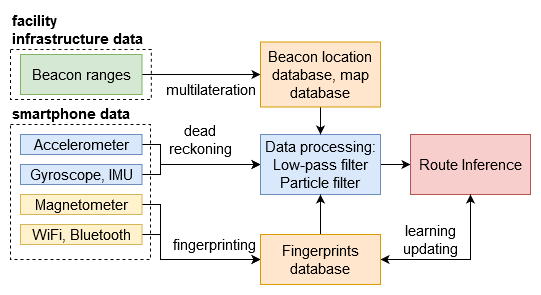
\includegraphics[width=0.48\textwidth]{img/indoor navigation roadmap-Page-3.png}
    \caption{Signal processing system architecture}
    \label{fig:arch}
\end{figure}

On figure \ref{fig:arch} we present possible architecture of indoor positioning application.
We use blue color for dead-reckoning application. Because of different smartphone sensors, signal processing will be different for every smartphone model, that's why signal processing should be done on the smartphone itself.

After first signal filtering from inertial and others complementary sensors (barometer), all information from sensors has to be matched with fingerprint database and map databases. This process can be done on the remote server or locally, this depends on system architecture chosen.

The technology choice of system architecture can't be explained, because there is no single strategy for system design.

Only several assumptions can be presented:

\begin{itemize}[noitemsep]
\item Server based systems can be provided by an external vendor - buying a service
\item Server based systems are enough cost effective to be used (development of server platforms in 2020 is enough to not care about signal processing on the local devices)
\item Mobile device based are harder in development and support
\item Mobile device based systems may not require external server and can be run locally - stable work with no internet connection
\item Once operating, mobile device based are cheaper, because no server support and rent needed - costs are on user side. Important for scalability (if one million of users will use system, some additional traffic management will be required)
\item Emergency help services shall not depend on internet connection - broadcast systems, mobile device used as transmitter - mobile device initiated systems
\item In some cases network initiated positioning can be useful. For example, if ultrasound waves are used for positioning, sound transmission will happen over short periods of time defined by network, this will reduce level of noise.
\end{itemize}

For the most common case of human tracking with no special requirements on internet connection, scalability and sensors used, architecture shown of \ref{fig:arch} can be used.

\begin{figure}[h]
    \centering
    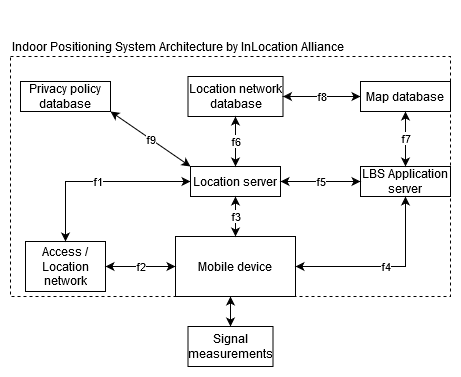
\includegraphics[width=0.48\textwidth]{img/InLocation Alliance (ILA).png}
    \caption{InLocation Alliance (ILA) system architecture}
    \label{fig:arch2}
\end{figure}

InLocation Alliance (ILA) was founded in 2012 and worked on indoor positioning solutions. In 2014 the ILA created an open, technology-independent architecture in support of accurate location of mobile devices within different types of indoor venues (see Figure \ref{fig:arch2}), which presents seven key system elements and nine interfaces.

What we see from Figure \ref{fig:arch2}, is that only mobile devices are considered as input, current architecture don't have beacons in it.

Results of ILA work and standards they make are not open and published, so they are not a standard now and we may freely update this structure.
Moreover, in \cite{Security} author propose to define both system architecture diagrams \ref{fig:arch} and \ref{fig:arch2} and use them as a product documentation to describe interfaces and so on.

% The ILA System Architecture (SA) specifies the main components and interface requirements of a technology-independent system architecture for indoor location.

% The SA has been designed to support a wide range of venues: from the very small (e.g. stand-alone business) to the very large (e.g. corporate campus) to the very distributed (e.g. worldwide retail chain).
% The SA is based on open interfaces in order to support multi-vendor environments for indoor location.
% While the SA in itself is generic and technology agnostic, the focus of the first public release of the SA is on Wi-Fi and BT.

\subsubsection{Roadmap system modelling}
% \subsubsection{Roadmap model in OPM}

From \cite{Security}, the process of documenting architecture can be described as:

At the appropriate times, take steps with prospective system providers:
\begin{itemize}[noitemsep]
\item Provide the two architecture diagrams to prospective vendors
\item Ask vendors to document the architecture and positioning mode(s) of the IPS being considered, relative to these architecture diagrams.
\item Plan and document any data import or export functions.
\item Review the existing system’s reporting capabilities against \ what reporting requirements apply for business uses of the system.
\item Review what applications reside where, such as an on-premises server or a cloud server.
\end{itemize}

We will create an OPM model using this approach and Figures \ref{fig:arch} and \ref{fig:arch2}.

\begin{figure*}[h]
    \centering
    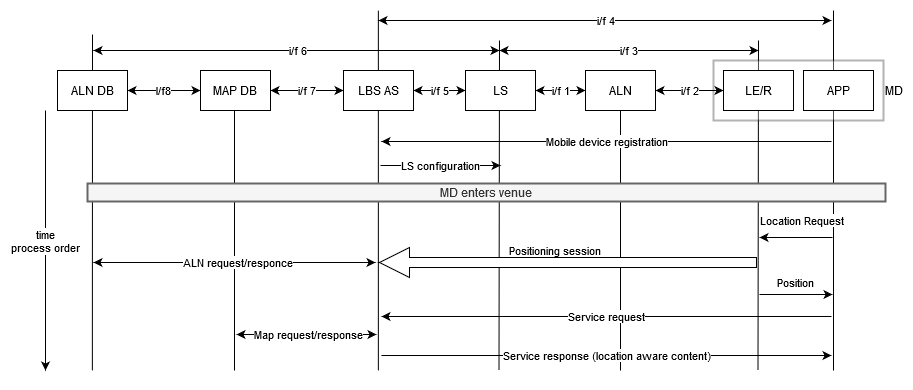
\includegraphics[width=\textwidth]{img/location aware content by ILA.png}
    \caption{Location aware content example by ILA.}
    \label{fig:loc_aware}
\end{figure*}

We present an example from \cite{ILA-System-Architecture} of how location aware content is delivered to users.
On Figure \ref{fig:loc_aware}, we see the order of steps, used to provide location aware content to user, e.g. geo-targeting or geo-fencing. This diagram doesn't explain much the structure and interfaces of system architecture, but shows some connections between them. All short naming are the same as in Figure \ref{fig:arch2}.

% For better structure representation we will use OPM models.



\subsection{Technology Strategy Vision}

% explain vision and strategy

From annual reports\cite{trends2017,trends2019} we can get history of trends in mobile marketing. When and where it is possible,different technologies and services are implemented in IPS. We will list several trends of indoor positioning systems.


Merge of indoor and outdoor positioning systems:
It is visible that IPS technologies are converging to some set of technologies. When this will happen, the connection between IPS and GPS or other outdoor positioning systems can be done. Right now, several IPS products support this feature, but this is not a global solution.\cite{Brena2017}
Privacy and security in IPS development:
Current trends with protection of users in web (GDPR policies) bring us to the point that some steps in this direction are done by government. Development of a product which is privacy safe can improve the adoption of use, which is important factor now. This factor directly affects the scalability of specific technologies and products.\cite{Brena2017}
Crowd-source mapping:
Most of technologies used in IPS systems requires hours of measurements inside the facilities to create a map of a building. Regular users can provide big amount of measurements, needed to create map of building and update it regularly.  This approach is important for applications that don't require special equipment for measurements and need regular map update (magnetic fields, WiFi, ambient sound localization technologies).\cite{Brena2017}
"China Crisis Ebbs, But Tracking Apps Are Going Strong" - the article of today's paper in The New York Times \cite{Tracking_Apps_times}.
Having the great need of tracking people, new products of human tracking were developed rapidly. "But the authorities have set few limits on how that data can be used. And now,officials in some places are loading their apps with new features, hoping the software will live on as more than just an emergency measure."
Indoor Location of E911 Mobile Callers:
Enhanced 911 Services enable 911 operators to:
Immediately pinpoint the location of the 911 caller based on the calling number
Callback the 911 caller if a disconnect occurs
Tracking location of people in emergency situation is an important challenge and one of the most important drivers of current IPS technology.
The initiative shown some results in 2013, but USA government requires universal service that will be implemented across the USA. One of the key points of this measure, that it has to work indoors. Importance of E911 point is that several actions are already done and several technological steps may change the state of USA market which may happen in future 2-5 years.

The overall strategy is to deliver the product in least development time, while reaching the average accuracy.

\subsection{Timeline}

We use data of Microsoft competition as a starting reference. In table \ref{tab:my-competition}, we have time of development and resulting accuracy for the different technology choice of different teams participated.
We may use these dependencies to understand, what time is needed to achieve each level of accuracy for different combinations of technologies.

\begin{figure}
  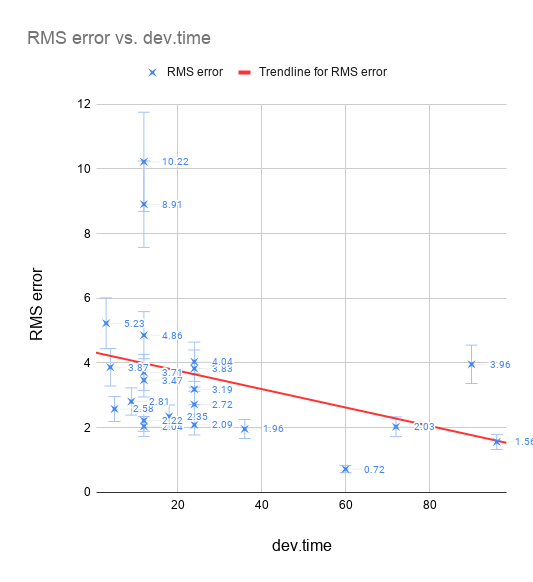
\includegraphics[width=0.49\textwidth]{img/RMSerrorvsdevtime.png}
  \caption{Root mean square error of positioning versus time of development}
  \label{im:rmse}
\end{figure}

On figure \ref{im:rmse}, we see the team competitors performance versus time for development in months.

\begin{table}[]
\caption{Technology choice.}
\label{tab:best-tech}
\begin{tabular}{lll}
Technical Approach & dev.time & RMS error \\
SDR Time-of-Flight & 4 & 3.87 \\
2.4GHz Time-of-Flight & 5 & 2.58 \\
WiFi+IMU Fingerprinting & 9 & 2.81 \\
WiFi+Modulated LEDs & 12 & 2.04 \\
WiFi Fingerprinting + Neural Network & 12 & 2.22 \\
WiFi+IMU Fingerprinting + Neural Network & 36 & 1.96 \\
2.4GHz Phase Offset & 60 & 0.72 \\
Bayesian Filter + WiFi Fingerprinting & 96 & 1.56
\end{tabular}%
\end{table}

We choose the best performance in technologies \ref{tab:best-tech} by multiplication of all of parameters.
Performance = 1 / (development time * accuracy).

We predict the accuracy of or product in between of optimal scenario (non-dominated points) and the trend line. From this we may present a timeline.

\begin{figure*}[t]
    \centering
    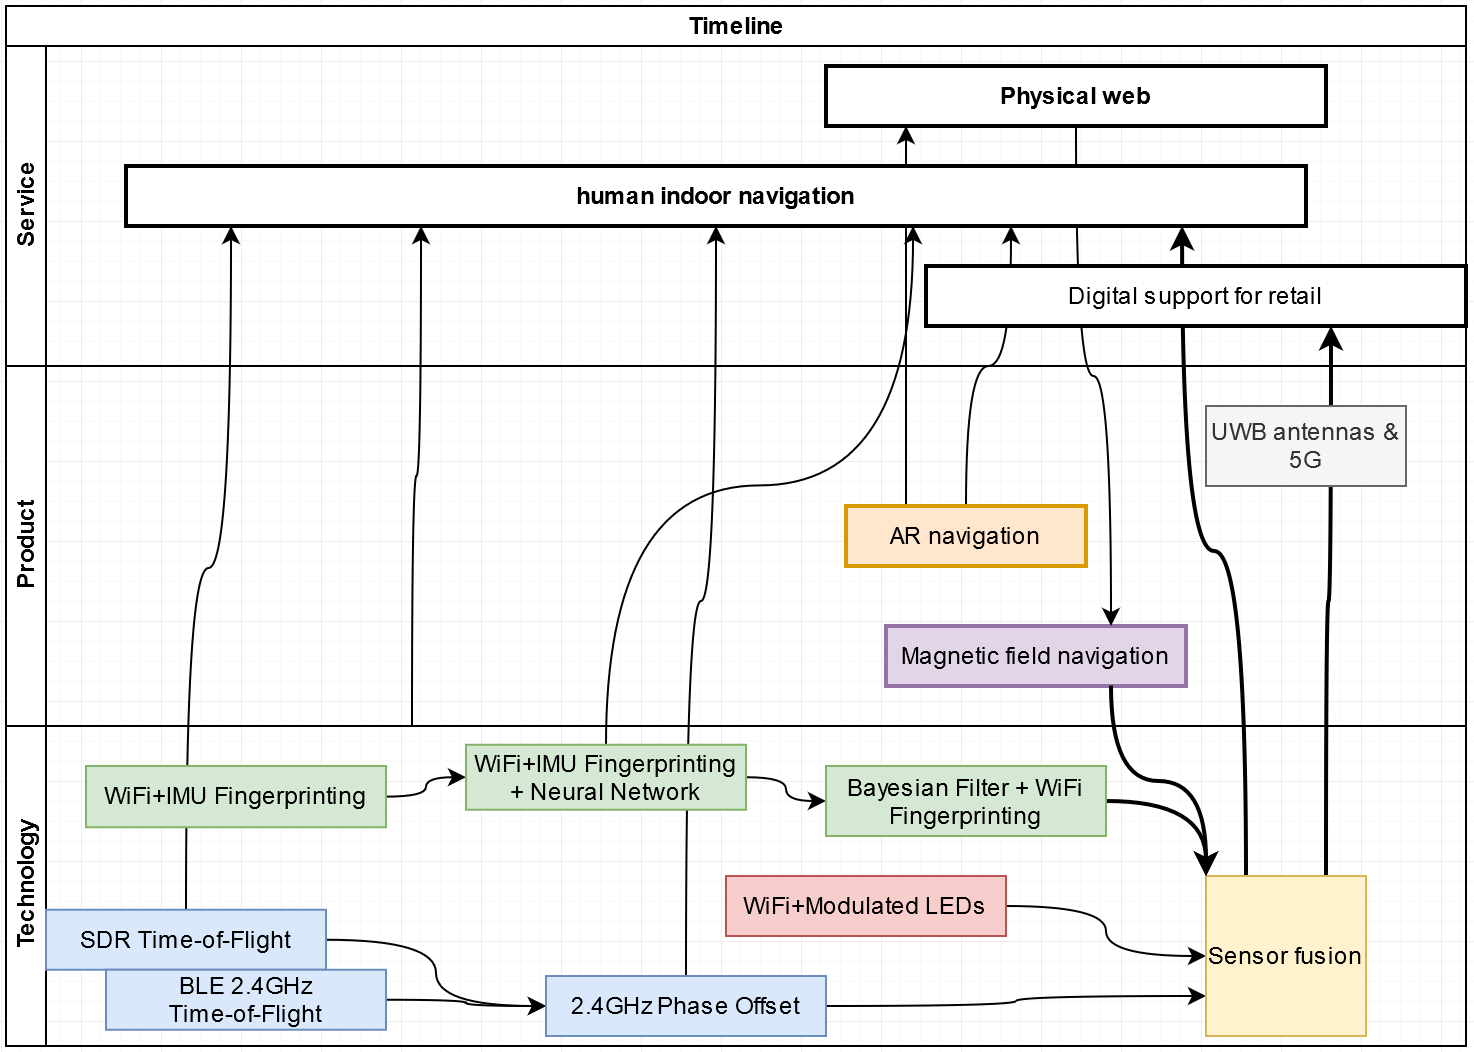
\includegraphics[width=0.9\textwidth]{img/timeline.png}
    \caption{Timeline diagram. Left to right: Passed term, Short term (1-2 years), Long term (2-5 years).}
    \label{fig:timeline}
\end{figure*}

On \ref{fig:timeline} we show the action plan for development the product with different alternative strategies.
 % historical evolution of trends in mobile technologies and technologies of indoor positioning.

The overall trend is that IPS products are converging to a global ecosystem - digitisation of cities. After human and assets will be tracked constantly, this will be a big supplementation to a smart cities technologies.
Before that, there is the market of IPS in retail applications (asset tracking, geo-fencing, way finding, proximity marketing).\cite{Infsoft_wp}

By speaking of current situation on the market, we can say that human indoor tracking is growing, but it is not mature.
We are building product with the main function of human indoor positioning as shown on Figure\ref{fig:timeline}.

Magnetic field navigation is another perspective factor in the timeline, some progress is already achieved by IndoorAtlas company in this field, but this technology will might become global and will assist the usual dead reckoning and existing WiFi and BLE technologies.

UWB localisation can be better than existing radio-based technologies, but until there is no UWB communication equipment in smartphones and facilities worldwide. Spreading of 5G may change this situation.
%
% The matchmaking apps are stated in the timeline, because it is the interest of current paper product research. This is the way of usage the IPS technology which merges social networks and geo-based services.
% \begin{wrapfigure}{l}{0.7\linewidth}
% 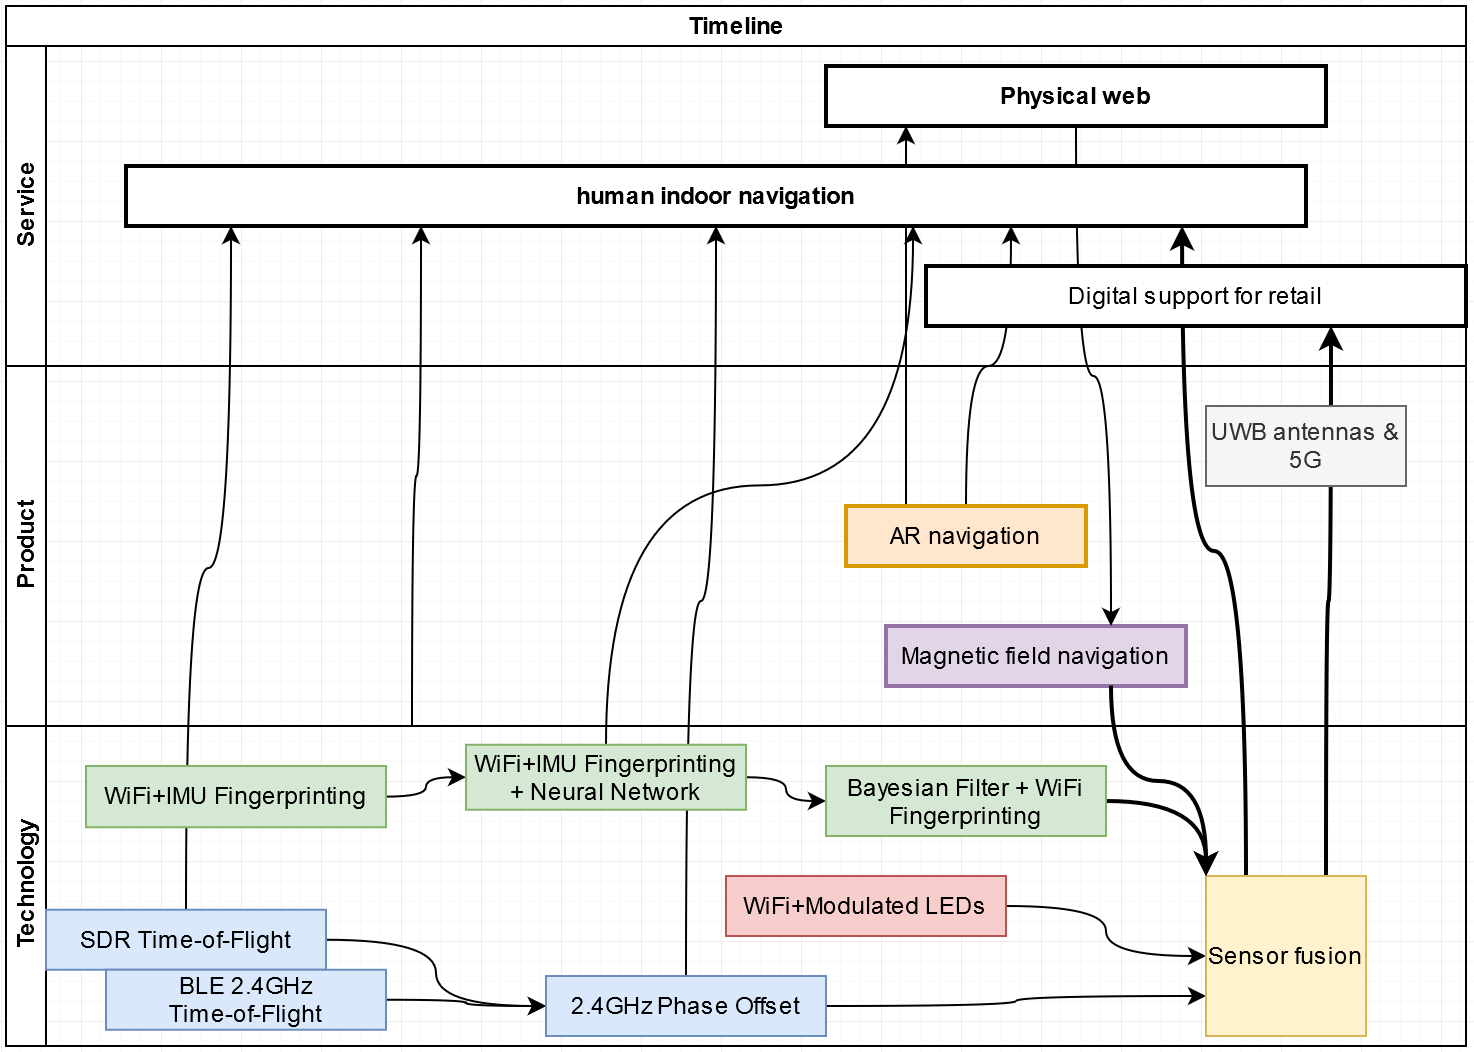
\includegraphics[width=\linewidth]{img/timeline.png}
% \caption{This is the former Share\LaTeX{} logo}
% \end{wrapfigure}
% To present current landscape, we will state known trends of this field.
% Because of uncertainty behind this information, in timeline they all can be marked under "Future applications".

\subsection{Technical feasibility}

Physical limits of indoor positioning system come from the environment. Real usage limits are more flexible and are directed by human limits (reaction time).

Applicable limits of each of FOM-s are different for different applications. For people to navigate, the accuracy of (1 m) and response frequency of (5 s)  may be enough. In big environment, the accuracy of 1-3 meters (similar to GPS performance) is enough. For the high performance applications, the accuracy must be lower than 1m (0.1 -0.5)m and response frequency near (0.1-0.5)s. In ARkit research[1] proposed model, where accuracy required is equal to 10 percent of the distance between various points of the destination, which gives us same 0.4-0.5m for rooms and 4-5m for big halls.


The range for RSSI method is calculated by formula:

$\mathbf{ dist = 10 * ((RSSI_{1m} - RSSI_{rec})/(10 * Path loss)) }$

Main limitation with this type of distance calculation is sensor's sensitivity and field noise. Having -96 DBm sensitivity and 4 DBm transmit power, system will be operable in range of 30m.

\begin{figure}
  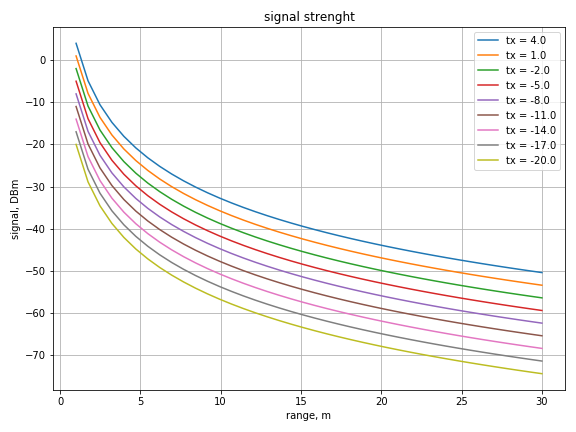
\includegraphics[width=0.49\textwidth]{img/signal_strenght.png}
  \caption{Radio signal strength distribution model.}
  \label{fig:signal}
\end{figure}
To calculate the signal distribution, we use Free-space path loss formula and Log-distance path loss model.

We use constants from signal measurements in [21], and Log-distance path loss model.

This gives us the information that signal transmission quality depends of distance, transmitter power and receiver sensitivity.

For BLE, we the normal conditions are as in figure above: with normal operating range of 30m, transmitter power in [4 DBm, -20 DBm] range, receiver sensitivity in range of -40 DBm, -60 DBm.

The limits for tracking technologies are not strict, they are only affecting accuracy and precision of localization. We can use table of normal ranges for technologies as a reference, but the performance will depend of huge amount of factors which can't be modeled accurately.

\subsection{Financial Valuation}

Customer Acquisition Cost (CAC)= (product cost+sales+marketing)÷(number of customers)

Life-Time Value (LTV) = (average value of sales) × (number of repeat transactions) × (average retention time)

Profit= LTV×(average margin)

Assumptions: 

\begin{enumerate}
    \item     an exhibition area of 1000 sqm, needs 9 BLE anchors for full coverage
    \item     Calculations for 1 day
    \item     1000 visitors per day
    \item     Mobile app development needs 4hrs of programming
    \item     1 person for hardware installation and removal
\end{enumerate}

Assumptions on revenues rate are shown on the figure above.

Plan A:

CAC~a~ to charge each booth (participating company) to benefit from indoor navigation facilities per day

Daily costs of operation = 1200 USD; Fixed costs = 3000 USD;

Plan B:

CAC~B~to charge each booth (participating company) to benefit from indoor navigation facilities + additional product features

Daily costs of operation = 1700 USD; Fixed costs = 2000 USD;

% \begin{figure}
%   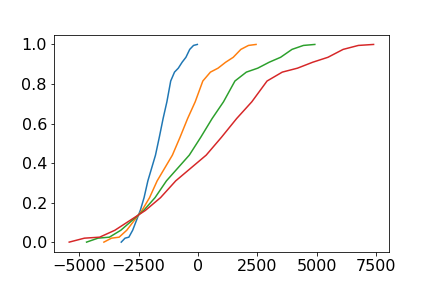
\includegraphics[width=0.49\textwidth]{img/fin/plan a.png}
%   \caption{Radio signal strength distribution model.}
%   \label{fig:signal}
% \end{figure}

\begin{figure}
  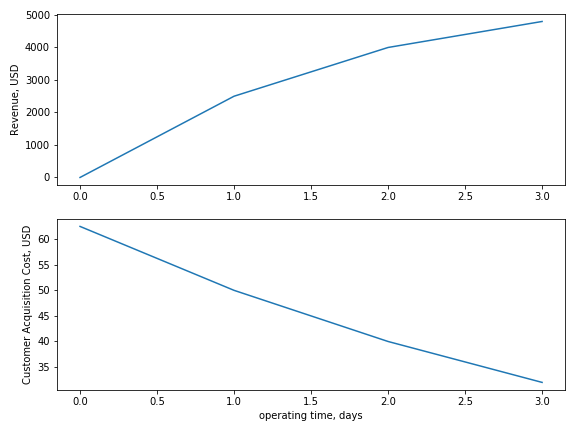
\includegraphics[width=0.49\textwidth]{img/fin/varg_10runs.png}
  \caption{Customer acquisition cost}
  \label{fig:cac}
\end{figure}

We assume that in strategies, CAC is different, and costs are different. Number of customers is assumed probabilistic as a triangular distribution. We use the assumption in the model, that for the longer operation time, customers get a discount as a power function of power 0.8.

The total revenue and customer acquisition cost are presented on the Figure \ref{fig:cac}. This is an example for one strategy, average customer acquisition is about 45 USD per day. Average revenue is about 1800 USD per day.

%We are modelling two strategies for operating time of 2 and 5 days.
%Watching on the figure, we understand that strategy A is better on a short term, and on a long operating time, both strategies are almost equal.


\begin{figure}
  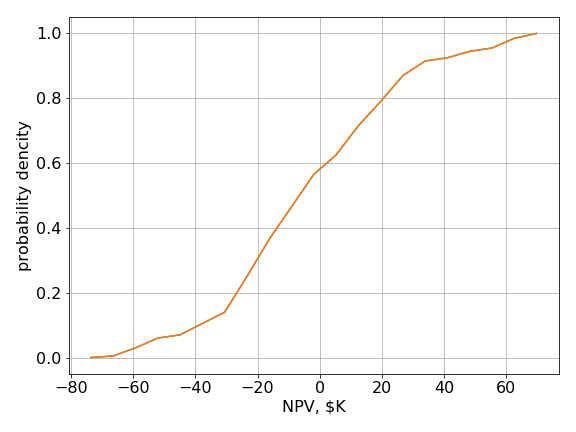
\includegraphics[width=0.49\textwidth]{img/fin/varg_mruns.png}
  \caption{Value at risk gain curve}
  \label{fig:signal}
\end{figure}

\section{Validation}


The tech background is validated by comparison of scientific publications \cite{ILA-System-Architecture}, \cite{Brena2017, Kj_fingerprinting, Li_geomagnetic, Mautz2012IndoorPT, AI-Centric_IPS} and analysis of the existing solutions.
The business model was sequentially developed to satisfy four fits model.
Expert validation (IndoorAtlas expert interview, customer interview).

One of the most valuable tools for the roadmap developing was benchmarking with existing researches \cite{microsoft}.
